\documentclass[a4paper,11pt,oneside,openright,xcolor=dvipsnames]{report}
\pdfminorversion=7

\usepackage[deliverable,history]{SecureCloud}
\usepackage{pdflscape}
\usepackage[hidelinks]{hyperref}
\usepackage{ulem}
\usepackage[latin1]{inputenc}
\usepackage{ifthen}
\usepackage{algorithm}
\usepackage{listings}

% define YAML style
\definecolor{darkgray}{rgb}{0.5,0.5,0.5}
\definecolor{darkgreen}{rgb}{0.3,0.5,0.3}
\definecolor{darkblue}{rgb}{0.3,0.3,0.5}
\definecolor{darkred}{rgb}{0.5,0.3,0.3}

\newcommand\YAMLcolonstyle{\color{darkred}\bfseries}
\newcommand\YAMLkeystyle{\color{darkblue}\bfseries}
\newcommand\YAMLvaluestyle{\color{darkgray}\bfseries}

\lstdefinelanguage{YAML}{
  keywords={true,false,null,y,n},
  keywordstyle=\color{darkgreen}\bfseries,
  basicstyle=\YAMLkeystyle,
  sensitive=false,
  comment=[l]{\#},
  morecomment=[s]{/*}{*/},
  commentstyle=\color{purple}\ttfamily,
  stringstyle=\YAMLvaluestyle\ttfamily,
  moredelim=[l][\color{orange}]{\&},
  moredelim=[l][\color{magenta}]{*},
  moredelim=**[il][\YAMLcolonstyle{:}\YAMLvaluestyle]{:},   % switch to value style at :
  morestring=[b]',
  morestring=[b]",
  literate =    {---}{{\ProcessThreeDashes}}3
                {>}{{\textcolor{red}\textgreater}}1
                {|}{{\textcolor{red}\textbar}}1
                {\ -\ }{{\mdseries\ -\ }}3,
}
% END define YAML style

\newboolean{shownotes}
\setboolean{shownotes}{true}
% \setboolean{shownotes}{false}
\ifthenelse{\boolean{shownotes}}
{ \newcommand{\citenote}[1]{\begin{quote}{\itshape\color{gray}#1}\end{quote}}}
{ \newcommand{\citenote}[1]{}}

\hyphenpenalty=2000
\tolerance=1000

\SECtitle{Specification and design of the scheduling for distributed big data applications}
\SECidentifier{D4.3}
\SECdueDate{... 2017}
\SECsubmissionDate{... 2017}
\SECresubmissionDate{... 2017}
\SECeditor{Pascal Felber}{UniNE}
%\SECcontributors{All}
\SECworkPackage{WP4}
\SECdissLevelPU
\SECreviewerone{...}{...}
\SECreviewertwo{...}{...}
\SECtask{...}{...}{UniNE$^*$}
\SECrevision{0.1}{2017/07/17}{Aur\'{e}lien Havet}{UniNE}{First draft}

\fancyhead[RO,LE]{\thepage}
\renewcommand{\headrulewidth}{0.4pt}

\sloppy

\begin{document}

\setcounter{tocdepth}{2}
\setcounter{page}{1}
\pagenumbering{roman}

\tableofcontents

\listoffigures

%\fancyhead{} % clear all header fields
\fancyhead[RO,LE]{\sffamily\bfseries Secure Big Data Processing in Untrusted Clouds}
\fancyhead[LO,RE]{\sffamily\bfseries Deliverable 4.3}
\fancyhead[LO,RE]{\sffamily\bfseries First Revision}
%\fancyfoot{} % clear all footer fields
\fancyfoot[CO,CE]{\thepage}

\setcounter{page}{1}
\pagenumbering{arabic}

\glsresetall

\renewcommand{\emph}[1]{\textbf{#1}}

\newcommand{\GP}{\textsc{GenPack}\xspace}

\newcommand{\testbedrepo}{\url{https://bitbucket.org/GenPackTeam/genpack-testbed}}
\newcommand{\remoteswarmmanagerrepo}{\url{https://bitbucket.org/GenPackTeam/remote-swarm-manager}}
\newcommand{\genpackschedulerrepo}{\url{https://bitbucket.org/GenPackTeam/genpack-scheduler}}


% -*- root: Document.tex -*-

\chapter{Introduction}
\label{chap:introduction}

\citenote{
This work package aims at designing and implementing building blocks for developing big data
applications on top of microservices (WP3), themselves deployed within containers (WP2) in the
cloud. The main objectives are to make the development of cloud-based big data application easier,
safer, and faster. More specifically, the work package will result in the following outcomes:
T4.1: Secure and efficient (i.e., low latency and high throughput) communication mechanisms for
transmitting big data between microservices, and between clients and big data applications.
T4.2: A secure distributed key/value data store for big data application to store their data, and
used by the map/reduce framework of T4.4 to store (intermediary) computation results.
T4.3: Distributed scheduling mechanisms designed for executing computation tasks (running in
microservices) close to the data they depend on, and for placing data close to associated compute
tasks or to related data for better efficiency.
T4.4: A generic framework for map/reduce computations with big data across microservices, as
well as a collection of pre-defined components for big data processing.
This workpackage is led by UniNE, with significant technical contributions from TUD, IMP, and CC.
}


Resource allocation in cloud data centers is an important yet complicated problem.
On the one hand, over-provisioning tends to waste resources---be they monetary or environmental.
On the other hand, overbooking yields poor performance and may lead to \emph{service level agreement} (SLA) violations, which also has financial consequences.

To increase the flexibility of task management, cloud data centers largely rely on virtualization to run applications and services for their customers.
While some providers offer dedicated servers at a premium price, most usually they co-locate several services and/or jobs on the same physical servers in order to optimize the use of available resources and reduce the associated costs.

Efficient mapping of services and jobs---packaged as system containers---to hosts is non-trivial as it should take into account, not only the resources available on the possibly heterogeneous machines, but also the properties and requirements of the containers.
For instance, some containers might require much memory but little CPU or I/O resources, while others are CPU-intensive, or primarily perform network and disk accesses.
To make the problem worse, these properties and requirements are not necessarily known in advance and must be learned at runtime.

In this document, we therefore introduce \GP, a novel scheduling framework for containers placement and migration in cloud data centers, which leverages principles from generational \emph{garbage collection} (GC)~\cite{Ungar:1984:GSN:390011.808261,Lieberman:1983:RGC:358141.358147}.
The core idea of \GP is to partition the servers into several groups, named \emph{generations}.
A first generation of servers, the \emph{nursery} generation, hosts new containers whose workload are not known.
There, the system containers are automatically monitored to determine their resource profile on reference machines in order to learn their characteristics.
To that end, we designed a monitoring framework that combines local statistics and power estimations from the \textsc{cAdvisor}~\cite{cAdvisor} and \textsc{BitWatts}~\cite{DBLP:conf/eurosys/ColmantKFHRS15} agents.

Once their workload is properly understood, the system containers are migrated to a server of the second generation, the \emph{young} generation.
The placement of system containers in the \emph{young} generation is performed according to resource-aware scheduling policies, and the servers in this generation are in charge of hosting containers whose lifetime is relatively short or unknown.

Finally, if a container runs for long enough in the young generation, it will be migrated to the \emph{old} generation.
Servers in this last generation are the most stable and tend to host long-term containers.
Placement is performed so as to optimize the load of the machines by co-locating containers that have complementary resource requirements.
For instance, a node that has high CPU utilization, but underloaded memory, will be candidate to host a memory-intensive container with low CPU requirements.

\GP allows us to take advantage of the different properties of the server generations and the system containers that they host to flexibly provision resources and thus save energy.
New machines can be added to each generation as needed.
This allows us to elastically adapt to demand and load variations---\emph{e.g.}, between day and night---and take advantage of server-specific properties---\emph{e.g.}, use the most energy-efficient machines for the old generation.
Furthermore, by rationalizing the usage of some servers while shutting down others, one can reach closer to \emph{energy-proportional computing}~\cite{Barroso:2007:Energy:Proportional:Computing}.

\GP provides several key original features: it supports heterogeneous data centers and servers with different properties (\emph{e.g.}, single- vs. multi-core, energy-efficient vs. fast, with or without HW acceleration, etc.); it supports containers whose workload and duration are not known in advance (which is the general case for many application domains) and must be learned at runtime; it supports fluctuating workloads by adapting the number of servers in the different generations, integrating fine-grained power estimation mechanisms, it supports thus enabling energy-efficient container scheduling in cloud data centers.

We have implemented our approach within the \textsc{Docker Swarm} framework~\cite{swarm}.
In particular, \GP includes a comprehensive monitoring framework, as well as resource management, container migration, and scheduling mechanisms.
We have tested our system in a dedicated data center with real-world traces from~\cite{DBLP:conf/eurosys/VermaPKOTW15}.
Our evaluation reveals that \GP is up to 23\% more energy-efficient than \textsc{Swarm}'s built-in schedulers with a real-world trace.

% -*- root: Document.tex -*-

\chapter{State-of-the-Art}
\label{chap:soa}

Resource management and scheduling is an important topic.
Many researchers have addressed various aspects of scheduling resources during the last decades.
Scheduling has been addressed in the context of GRID computing~\cite{buyya2000nimrod}, distributed systems~\cite{tannenbaum2001condor}, HPC~\cite{Jackson2001}, batch processing~\cite{capit2005batch}, MapReduce~\cite{Yarn}, and more recently in the context of VM~\cite{litvinski2013openstack} and container scheduling~\cite{Burns:2016:BOK:2930840.2890784} in large clusters.

Distributed job schedulers like the \textsc{Condor} scheduler~\cite{tannenbaum2001condor} performs a \emph{match making} between a job waiting to run and the machines available to run jobs.
Hence, each job explicitly describes its resource requirements and also a \emph{rank expression} that permits the scheduler to select the machine that is most suited to run this job.
Also, the resources of a machine have to be explicitly described.
In \GP, we avoid the need to describe jobs and machines by performing an automatic profiling of the containers and nodes (cf. Section~\ref{sec:monitoring}).

The \textsc{OpenStack Nova} scheduler does not consider CPU load for the assignment of VMs~\cite{litvinski2013openstack}.
The scheduling in \textsc{OpenStack}, no matter the selected strategy, is rather based on statically defined RAM and CPU size of the VM, known as flavors~\cite{litvinski2013openstack}.
In our experience, the simple round-robin scheduler results in many cases in situations where all hosts run some VMs and none of the hosts can be switched off to reduce the energy consumption (cf. Chapter~\ref{chap:motivation}).

\textsc{OptSched}\cite{knauth2012energy} compares the energy implications of a \emph{round robin} scheduler, a \emph{first fit} scheduler, and an \emph{optimized} scheduler that knows the run time of (some of) the VMs upon scheduling.
Knowing the run times before starting a VM helps reduce the total energy consumed by a cluster.
In \GP, however, run times are not known \emph{a priori} and \GP is able to automatically learn the profile that is used by the scheduler along generations to improve the energy efficiency of the cluster (cf. Section~\ref{sec:evaluation}).

\textsc{Yarn}~\cite{Yarn} is a two-level scheduler that can handle multiple workloads on the same cluster.
It is request-based and supports locality of scheduling decisions such that jobs can, for example, access data on local disks to avoid remote accesses via the network.
Nonetheless, the scheduling in \textsc{Yarn} implements a strategy close to the \emph{spread} strategy of \textsc{Docker Swarm}, thus suffering from the same limitations in terms of power usage efficiency.

Google developed a series of container management systems during the last 10 years~\cite{Burns:2016:BOK:2930840.2890784}: \textsc{Borg}, \textsc{Omega}, and more recently \textsc{Kubernetes}.
Initially, Google started with a centralized container management system called \textsc{Borg}, which remains the main system in use by Google~\cite{DBLP:conf/eurosys/VermaPKOTW15}.
\textsc{Omega} is based on the lessons learned from \textsc{Borg} and has a principled architecture that includes a centralized transactional store and an optimistic concurrency control.
In particular, the \textsc{Omega} architecture supports multiple concurrent schedulers.
Finally, \textsc{Kubernetes} is an open source container system that focuses on simplifying the task of application developers and has less focus on maximizing the utilization of clusters---which is the focus of \textsc{Omega} and \textsc{Borg}.
Compared to \GP{}, all these approaches does not incorporate the concept of generations within the cluster to automatically learn about the container profiles at runtime.

\textsc{Docker Swarm} is very similar to \textsc{Kubernetes} in that it aims to support \emph{cloud native} applications.
\textsc{Swarm} permits users to define applications consisting of a set of containers.
The focus is on simplifying the typical tasks of the application developers like load balancing, elasticity, and high availability.
Unlike \GP, the main goal of \text{Swarm} is not on ensuring a high utilization of a compute cluster, but this document demonstrates how we succeed to extend it in order to address this concern.

% -*- root: Document.tex -*-

\chapter{Motivating Scenario}
\label{chap:motivation}

To illustrate and assess the benefits of proper container (or VM)\footnote{In the remaining of this document, we primarily consider containers, which are essentially lightweight VMs, and we use the two terms interchangeably.} placement, we first illustrate the limitation of existing scheduling policies on a simple scenario.

We define two types of containers: \emph{cpu-heavy} containers require 2 CPU cores and 1\,GB of RAM, while \emph{mem-heavy} containers require only 1 CPU core but 2\,GB of RAM.
We set up a cluster of nodes with 8 available cores and 8\,GB of RAM, running \textsc{Ubuntu Server} (v15.10) and \textsc{Docker} (v1.10.1).
The containers are managed by \text{Docker Swarm} (v1.2.0) and they execute the \textsc{stress-ng} benchmark~\cite{stress-ng} with a fixed total number of operations before terminating.

We deploy the containers in a dedicated cluster using four placement strategies:
\begin{itemize}
  \item \texttt{spread} places new containers on the node with the least number of containers;
  \item \texttt{binpack} deploys containers on the same node until its resources are totally exhausted before moving to the next node;
  \item \texttt{random} dispatches containers at random;
  \item \texttt{custom} assigns containers to nodes so that they fit into the least number of nodes, by taking into account both the CPU and memory requirements.
\end{itemize}

\begin{figure}[t]
  \centering
  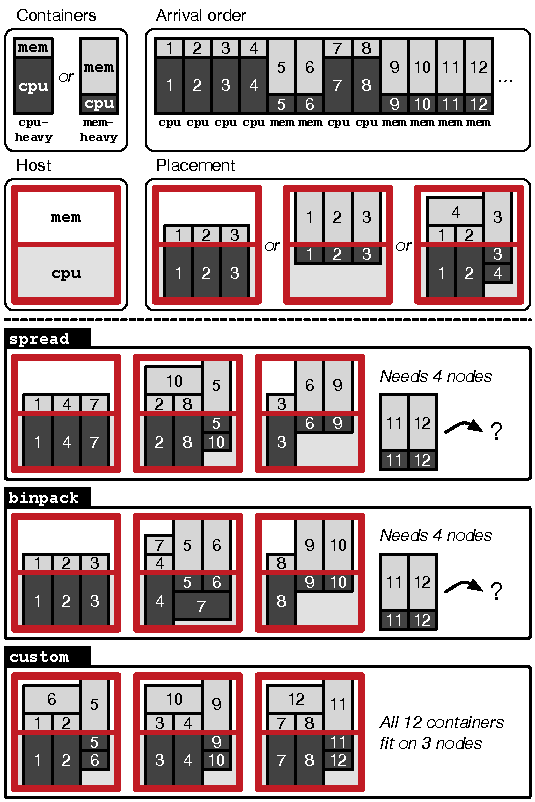
\includegraphics[width=.7\linewidth]{figures/scenario}
  \caption{Placement of the containers with 3 scheduling strategies for a given arrival order of containers, and assuming that a node can host 3 \emph{cpu-heavy} containers, or 3 \emph{mem-heavy} containers, or 2 of each type (top). While \texttt{spread} and \texttt{binpack} would require 4 nodes to schedule 12 containers, \texttt{custom} requires only 3 (bottom).}
  \label{fig:motivating-placement}
\end{figure}

For the sake of illustration, assume that a node can host \emph{(i)} 3 \emph{cpu-heavy}, or \emph{(ii)} 3 \emph{mem-heavy}, or \emph{(iii)} 2 \emph{cpu-heavy} and 2 \emph{mem-heavy} containers of each type.
In that case, a scheduler that takes into account the nature of the workload can obviously perform more efficient container placement.

Figure~\ref{fig:motivating-placement} shows a simple execution where the 12 containers (6 of each type) are registered in the following order: 4 \emph{cpu-heavy}, 2 \emph{mem-heavy}, 2 \emph{cpu-heavy}, 4 \emph{mem-heavy}.
Containers specify their resource needs and the system performs placement accordingly without overbooking.
A possible container scheduling for the \texttt{spread}, \texttt{binpack}, and \texttt{custom} strategies is shown in the bottom part of the figure.
As one can see, with 3 nodes available the first two strategies can only schedule 10 containers, whereas the \texttt{custom} strategy can place all of them on the 3 nodes.
Although very simplistic, this example illustrates the need for scheduling strategies that are aware of the requirements of the containers and the properties of the workloads.

\begin{figure}[t]
  \centering
  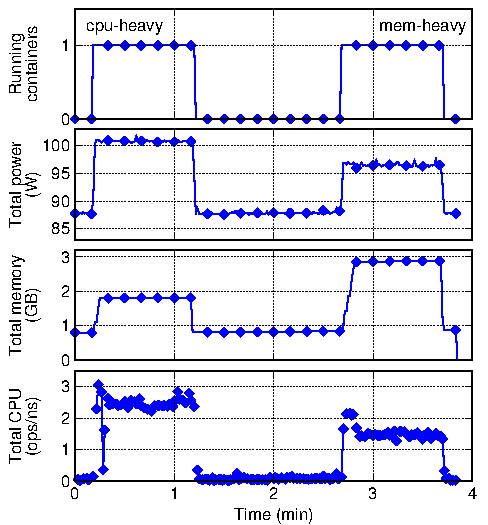
\includegraphics[width=.7\linewidth]{figures/plots/motivating_baseline/motivating_baseline}
  \caption{Workload for the two container types (\emph{cpu-heavy} and \emph{mem-heavy}) deployed on a single host.
  Each container runs for one minute, with an idle period in between.
  }
  \label{fig:motivating_baseline}
\end{figure}

In our actual experiment, we set the CPU load of containers to 20,000 ``bogo'' operations\footnote{Fake operations that represent the unit of load of the benchmark.} for each CPU core.
This corresponds to a total of $40,000$ and $20,000$ operations for \emph{cpu-heavy} and \emph{mem-heavy} containers, respectively.
Figure~\ref{fig:motivating_baseline} shows the baseline workloads induced by the two types of containers deployed on a single node, running one after the other within the span of $5$ minutes.
As expected, \emph{cpu-heavy} containers consume more energy---if we subtract the idle power, they require almost 50\% more than \emph{mem-heavy} containers---but they are less memory demanding.

Then, we design a more elaborated deployment scenario where we deploy start $20$ containers, alternating $5$ \emph{cpu-heavy} and $5$ \emph{mem-heavy}.
In all four deployment scenarios, we gather several measures (\emph{e.g.}, memory allocations, CPU usage, power consumptions).
Results are aggregated values over all nodes: number of CPU operations by time unit ($ns$), memory used in $GB$, and cumulative power (idle power and dynamic consumption) in $W$.
We observe that the \texttt{custom} strategy results in a more memory- and energy-efficient schedule because one of the nodes can be turned off---hence saving the idle power---without noticeably changing the number of operation executed---\emph{i.e.}, performance.

\begin{figure}[t]
  \centering
  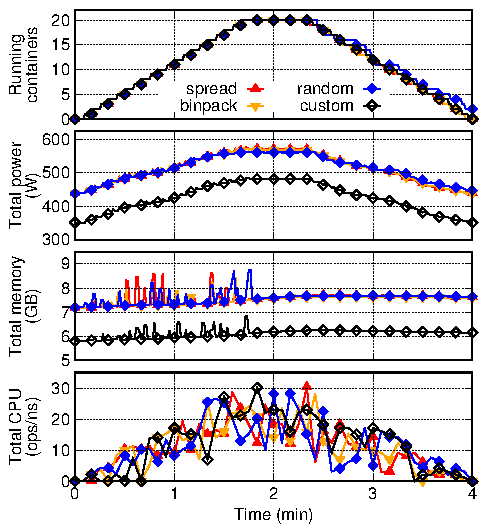
\includegraphics[width=.7\linewidth]{figures/plots/motivating/spread-binpack-random-custom}
  \caption{The \texttt{custom} strategy saves memory and energy without affecting performance thanks to more efficient container scheduling.}
  \label{fig:motivating}
\end{figure}

\newpage

As a summary, we aim at delivering a new container scheduler, \GP{}, that automatically learns from container's workloads to evenly distribute their deployment across a reduced number of nodes, thus drastically improving the power usage efficiency of a cluster.
As demonstrated, the state-of-the-art fails to achieve this objective as the \texttt{spread} strategy distributes the containers across all the nodes and \texttt{binpack} adopts a greedy heuristics to allocate containers node per node.
Given a set of available nodes $N$, we therefore aim at proposing a solution that minimizes the number of powered nodes required to host a set of containers $C$, thus ensuring that $|\text{genpack}(N,C)| \le |\text{binpack}(N,C)| \le |\text{spread}(N,C)| = |N|$, where $\text{f}(N,C)|$ indicates the number of nodes necessary for scheduling $C$ containers on $N$ nodes using algorithm $\text{f}$.
By doing so, \GP{} reduces the overall power consumption of a cluster without impacting the containers' performance, since hosts are not energy proportional (as shown in Figure~\ref{fig:motivating_baseline}).

% -*- root: Document.tex -*-

\chapter{\GP{} Architecture}
\label{chap:arch}

In this chapter, we provide an overview of the software architecture of \GP, as well as its main components and their interactions.
Further details about the implementation of these components and how they operate are given in the following sections.

% -*- root: Document.tex -*-

\section{Generations}
\label{sec:generations}

As previously mentioned, \GP splits the nodes of a cluster into multiple generations, each responsible for specific types of containers and tasks.
The rationale is that, by specializing nodes for a given type of workloads, one can handle system containers whose properties are not known in advance or are dynamically evolving, while at the same time optimize the whole system's efficiency by placing the containers on the most appropriate nodes.

Along the same lines as generational garbage collectors in managed languages, \GP considers 3 generations: the nursery, the young generation, and the old generation, as illustrated in Figure~\ref{fig:generations}.

\begin{figure}[H]
  \centering
  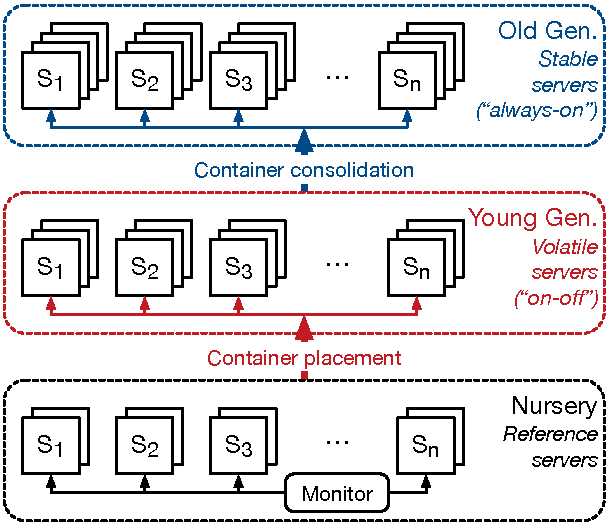
\includegraphics[width=.75\linewidth]{figures/architecture}
  \caption{\GP's different generations.}
  \label{fig:generations}
\end{figure}

% \newpage

The \emph{nursery} consists of a set of reference nodes that are representative of servers in the data center and whose properties are well understood.
A container that has not yet been profiled will first execute in the nursery.\footnote{Note that containers can skip the nursery and directly go to the next generation when previously profiled.}
During its first period of execution, \GP will monitor its resource requirements as well as its power consumption.
To that end, it leverages system-level metrics provided by \textsc{cAdvisor} (see \S\ref{sec:monitoring}) and power information from \textsc{BitWatts}~\cite{DBLP:conf/eurosys/ColmantKFHRS15}.
This observation phase allows \GP to establish a profile for the container.

Once a container's properties are known, and assuming that it did not complete its execution, it is moved to the \emph{young generation} (``placement'' phase) on a server that has sufficient resources available considering the container's specific requirements (CPU, memory, network, etc.).
The young generation hosts containers that have recently started their execution and whose lifetime is still unknown.
If the container survives long enough, it moves to the next generation.
The reasoning behind this placement strategy is that, similarly to in-memory data objects, a significant portion of the containers are expected to have a short lifetime.\footnote{We assess this statement in Section~\ref{sec:evaluation}.}
Furthermore, as the young generation is the most exposed to load variations (\textit{e.g.}, when many new containers are simultaneously launched), it will provide mechanisms for elastically scaling up and down, according to demand.
In particular, nodes can be completely turned off during periods of low load in order to considerably reduce the energy consumption of the cluster.

Finally, the \emph{old generation} consists of stable and power-efficient servers that host the long-running containers.
The placement of containers on the nodes (``consolidation'' phase) is performed in such a way that they occupy the minimum number of servers in order to optimize resource and power usage, as motivated in \S\ref{chap:motivation}.
Barring important workload variations, containers do not need to migrate further once they are on an old generation node.

The actual monitoring and scheduling operations that drive the migrations between generations are described in \S\ref{sec:monitoring} and \S\ref{sec:scheduling}.


\newpage

% -*- root: Document.tex -*-

\section{System components}
\label{sec:sys_components}

From a high-level perspective, \GP is composed of three main components:
\begin{itemize}
  \item The \emph{monitoring} module is responsible for keeping track of resources consumption in the system.
  \item The \emph{placement and migration} module handles the deployment of containers and their relocation to different nodes as they move across generations.
  \item The \emph{scheduling} module contains the algorithms that orchestrate and take decisions regarding container placement and migrations, based on the input received from the monitoring module.
\end{itemize}

The role and interactions between these components are schematically illustrated in Figure~\ref{fig:components}.

\begin{figure}[H]
  \centering
  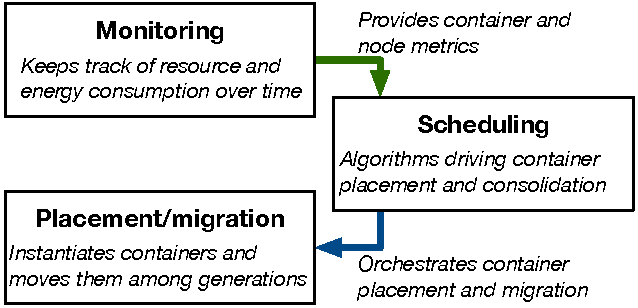
\includegraphics[]{figures/components}
  \caption{\GP's abstract components and their interactions.}
  \label{fig:components}
\end{figure}


% -*- root: Document.tex -*-

\chapter{\GP's components}
\label{chap:comp}

In this chapter, we detail the 2 main components of \GP{}:
\begin{itemize}
  \item the monitoring system needed for profiling container resources usages and achieved by \textsc{cAdvisor} and \textsc{InfluxDB};
  \item the scheduling mechanism responsible for containers optimized placement.
\end{itemize}

% -*- root: Document.tex -*-

\section{Container and Node Profiling}
\label{sec:monitoring}

System containers can exhibit a wide diversity of properties and requirements, from CPU-intensive tasks running for a short duration to longstanding memory-intensive applications serving user requests.
In such a context where the workloads are unknown, it is particularly challenging to ensure an efficient scheduling of these containers.
We therefore propose to introduce a resource profiling phase within \GP{} to automatically learn the resource requirements of a container during the beginning of its execution, and to subsequently use this information to compute a resource envelope that will help the \GP{} scheduler to appropriately place the container on the best fitting node for the rest of its execution.
In particular, this container profiling phase is performed within the \emph{nursery} and \emph{young} generations of \GP{} and is complemented with a monitoring of the nodes located in the \emph{young} and \emph{old} generations in order to maintain a up-to-date cartography of available resources in the cloud data center.

\paragraph{Profiling the resources consumption.}

Upon deployment of a new container within the \emph{nursery} generation, \GP{} uses a \textsc{cAdvisor} daemon~\cite{cAdvisor} to collect, aggregate, process, and export metrics about running containers every $30$ seconds.
In particular, \textsc{cAdvisor} logs resource isolation parameters, historical resource usage, histograms of complete historical resource usage, and network statistics for each system container running on a \textsc{Docker} host.
Collected metrics are automatically exported towards an \textsc{InfluxDB} service~\cite{influxdb} hosted on the master node (see Figure~\ref{fig:monitoring}).
\textsc{InfluxDB} provides a time-series database to store cluster-wide metrics per container, according to a specific data retention policy ($x$ minutes in \GP{}).
Whenever needed, \GP{} can therefore query \textsc{InfluxDB} to learn about the containers' workloads.

\begin{figure}[t]
\centering
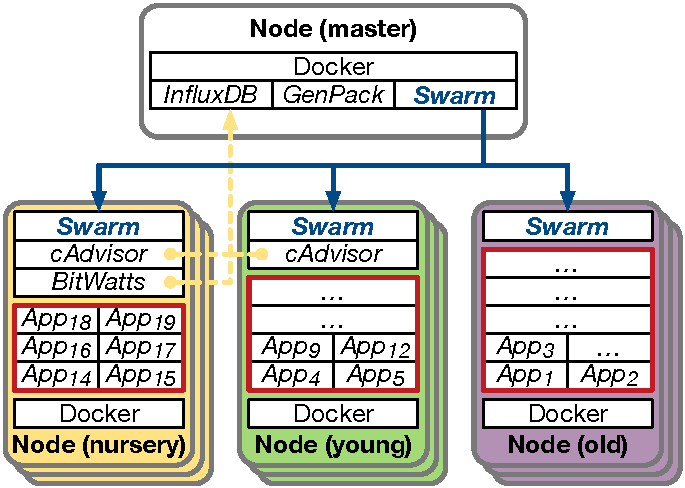
\includegraphics[width=.7\linewidth]{figures/monitoring}
\caption{Overview of the monitoring support in \GP{}.}
\label{fig:monitoring}
\end{figure}

\paragraph{Computing the container envelopes.}

Periodically, \GP{} picks the containers running in the \emph{nursery} generation and triggers a scheduling phase for all of them.
As part of this phase, \GP{} queries \textsc{InfluxDB} to convert raw resource metrics into \emph{container envelopes}, which will be used by the scheduler to estimate the expected resource consumption.
In particular, for each resource, \GP{} first computes the metrics distribution and extracts the \emph{$90^{\,th}$ percentile} value as a component of the resource envelope.
Then, \GP{} splits the set of containers into $k$ clusters by applying the \emph{k-means} algorithm, which belongs to the category of unsupervised learning approaches.
For example, we can set $k=4$ to segregate $4$ classes of CPU-, disk-, network-, and memory-intensive workloads into $4$ container envelopes.
% \cf{Intuitively this makes sense but is there some empirical evidence that k=4 is a good choice?}

Finally, within each envelope, containers are ordered per decreasing resource consumption score, which is computed for each enclosed container~$i$ as:
\small
\[score_i=\sqrt{(\frac{cpu_i}{\sum{cpu}})^2+(\frac{disk_i}{\sum{disk}})^2+(\frac{net_i}{\sum{net}})^2+(\frac{mem_i}{\sum{mem}})^2}\,.\]
\normalsize

The resulting container envelopes are posted to the \GP{} scheduler, which is in charge of placing the containers among the nodes of the \emph{young} generation.

\begin{figure}[t!]
	\centering
	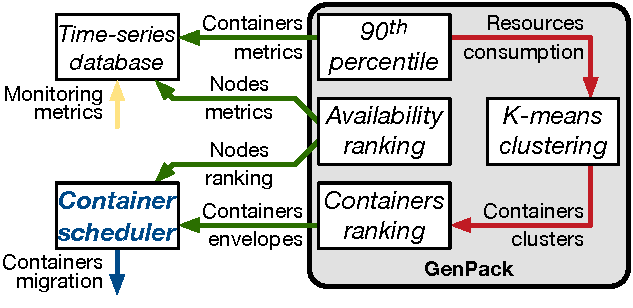
\includegraphics[width=.7\linewidth]{figures/profiling}
	\caption{Container and node profiling in \GP{}.}
	\label{fig:profiling}
\end{figure}

Beyond this first scheduling phase, \GP keeps monitoring and profiling the containers within the \emph{young} generation in order to consolidate the resource envelope prior to a later migration in the \emph{old generation}.

\paragraph{Maintaining the node availability cartography.}

\GP{} monitors the resource availability of nodes within the \emph{young} and \emph{old} generations.
For each generation, it uses this information to rank the nodes according to resource availability, least available nodes first, by computing for each node $j$ the availability level as:
\small
\[availability_j=\sqrt{cpu_{ratio}^2+disk_{ratio}^2+net_{ratio}^2+mem_{ratio}^2}\,,\]
\normalsize
\noindent which corresponds to the norm of the resource vector
$\vec{r_j}=\begin{matrix}(cpu_{ratio} & disk_{ratio} & net_{ratio} & mem_{ratio})\end{matrix}$
that \GP{} extracts from \textsc{InfluxDB}.
This ranking of nodes will then be used by the scheduler to find the first fitting node to host a container, ultimately minimizing the number of hosts to be used---\emph{i.e.}, that need to be powered up.


\newpage

% -*- root: Document.tex -*-

\section{Container Scheduling}
\label{sec:scheduling}

Once the container profiles are identified and the associated resource envelopes have been computed by the monitoring module of \GP{}, the scheduling module builds on these resources estimations to identify the best fitting node for each of the container executing in the \emph{nursery} generation.

\begin{algorithm}[ht!]
  \begin{algorithmic}[1]
    \Procedure{Schedule}{$envelopes$, $nodes$}
        \State $containers \gets \Call{Blend}{envelopes}$\label{alg:scheduling:blend}
        \For{$c \in containers$}
            \State $res_c \gets \Call{Resources}{$c$}$
            \For{$n \in nodes$}\Comment{Find the best node for $c$}\label{alg:scheduling:find-best-node}
                \State $avail_n \gets$ \Call{Availability}{$n$}
                \If{\Call{Matches}{$res_c$, $avail_n$}}\label{alg:scheduling:pick-best-node}%\Comment{$cont$ fits in $node$}
                    \State $n \gets$ \Call{Update}{$n$, $res_c$}\label{alg:scheduling:update-node}
                    \State $nodes \gets$ \Call{ShiftLeft}{$nodes$, $n$}\label{alg:scheduling:shift}
                    \State \Call{Migrate}{$c$, $n$}\Comment{Async. migration}\label{alg:scheduling:migrate}
                    \State \textbf{break}\Comment{$c$ succeeds to be scheduled}
                \EndIf
            \EndFor
            \State \Call{Escape}{$c$}\Comment{$c$ fails to be scheduled}\label{alg:scheduling:escape}
        \EndFor
    \EndProcedure
    \vspace{5pt}
    \Function{Blend}{$envelopes$}\label{alg:scheduling:blend-begin}
        \State $list \gets \{\}$
        \State $emptied \gets \textbf{true}$
        \Repeat\Comment{Blend until all envelopes are emptied}
            \State $emptied \gets \textbf{true}$
            \For{$env \in envelopes$}
                \If{\textbf{not} \Call{IsEmpty}{$env$}}
                    \State $list \gets list~\Vert~\Call{Head}{env}$ %\Comment{appends}
                    \State $env \gets \Call{Tail}{env}$ %\Comment{appends}
                    \State $emptied \gets \Call{IsEmpty}{$env$}$
                \EndIf
            \EndFor
        \Until{$emptied$}
        \State \Return $list$
    \EndFunction\label{alg:scheduling:blend-end}
    \vspace{5pt}
    \Function{ShiftLeft}{$nodes$, $node$}\label{alg:scheduling:shift-begin}
        \State $i \gets \Call{Index}{nodes, node}$
        \State $n \gets \Call{Length}{nodes}$
        \State $list \gets nodes[0:i-1]~\Vert~nodes[i+1:n-1]$
        \State $i \gets 0$
        \State $score \gets \Call{Availability}{node}$
        \While{$score \ge \Call{Availability}{list[i]}$}
            \State $i \gets i+1$
        \EndWhile
        \State \Return $list[0:i-1]~\Vert~node~\Vert~list[i:n-1]$
    \EndFunction\label{alg:scheduling:shift-end}
  \end{algorithmic}
  \caption{Container scheduling in \GP{}.}\label{alg:scheduling}
\end{algorithm}

More specifically, Algorithm~\ref{alg:scheduling} describes the scheduling strategy applied by \GP{} to migrate a set of profiled containers at runtime.
The scheduling phase is triggered for a given set of container $envelopes$ and available $nodes$.
The algorithm starts by homogeneously blending the content (\emph{i.e.}, container descriptions) of the envelopes (line~\ref{alg:scheduling:blend} and lines~\ref{alg:scheduling:blend-begin}--\ref{alg:scheduling:blend-end}) to increase of the diversity of containers per node.
From there, it iterates over this ordered set of $containers$ to be scheduled (line~\ref{alg:scheduling:find-best-node}) and picks the first node $n$ among the ordered list of available $nodes$ (as explained in the previous section) that matches the resources requirements of the container $c$ (line~\ref{alg:scheduling:pick-best-node}).
Upon resource matching, the estimation of the node's resource availability is updated accordingly (line~\ref{alg:scheduling:update-node}) and the order of available $nodes$ is refreshed by shifting the selected node $n$ towards the head of the ordered list (line~\ref{alg:scheduling:shift} and lines~\ref{alg:scheduling:shift-begin}--\ref{alg:scheduling:shift-end}).
By reasoning on such resources estimations, \GP{} can therefore trigger the migration of the container $c$ to the node $n$ asynchronously (line~\ref{alg:scheduling:migrate}) and thus keep scheduling the remaining nodes in parallel.
If none of the available $nodes$ fits the resource requirements of the container $c$, the escape trigger of \GP{} (line~\ref{alg:scheduling:escape}) is used to provision a new node within the \emph{young} generation, migrate the container $c$ on this new node, and add the node to the list of available nodes.

The intuition behind this algorithm is to ensure a better distribution of resource consumption and power efficiency of the infrastructure by increasing the entropy (in term of resource diversity) of the containers deployed within each node.
Furthermore, by reasoning on resource estimations (computed during the monitoring phase) instead of real-time metrics, \GP{} can increase the scheduling parallelism and thus absorb the delay induced by the container migration process (including state snapshotting, binary transfer, remote provisioning steps).


% -*- root: Document.tex -*-

\chapter{Proof of Concept}
\label{chap:poc}

\GP{}'s scheduling approach has been tested trough a proof-of-concept which has been experimented in IIUN's laboratory and which is detailed in this chapter.

% -*- root: Document.tex -*-

\section{Implementation}
\label{sec:implementation}

\textsc{Docker Swarm} is implemented in Go, but it offers multiple bindings for other programming languages.
We fully implement \GP in the Ruby programming language (v2.3.1).
In particular, we based our code on gem \emph{docker-api}~\cite{docker-api}, a lightweight Ruby binding for the \textsc{Docker Remote} API, using \textsc{Docker} API (v1.16)~\cite{docker-remote}, compliant with the one used by \textsc{Docker Swarm}(v1.22).
The scheduler orchestrates the containers by leveraging \textsc{Resque}~\cite{resque}, a \textsc{Redis}-backed Ruby library for creating background jobs.

In our evaluation, we map containers to jobs and rely on a \textsc{Resque}-based scheduler to timely deploy them over the \textsc{Docker Swarm}.
\GP is released as open-source and is freely available at \testbedrepo.


\newpage

% -*- root: Document.tex -*-

\section{Evaluation}
\label{sec:evaluation}

This section reports on a detailed evaluation of the \GP prototype.
More specifically, we describe our experimental settings in~\S\ref{subsec:eval:settings}.
\S\ref{subsec:eval:trace} characterizes the real-word trace used in our experiments, focusing in particular on the simplifications that we applied to make it applicable in our dedicated data center.
We present the performances of the \GP approach in terms of job completion and energy impact when compared against different default strategies in \S\ref{subsec:eval:compl} and \S\ref{subsec:eval:energy}, respectively.
Finally, \S\ref{subsec:eval:inside} offers an insider-view on the dynamics of the generations in terms of running containers.

\subsection{Evaluation settings}
\label{subsec:eval:settings}

We deploy and conduct our experiments over a cluster machines interconnected by a $1\,Gb/s$ switched network.
Each physical host features 8-Core Xeon CPUs and $8\,GB$ of RAM.
We deploy dedicated \emph{virtual machines} (VM) on top of the hosts.
The KVM hypervisor, which controls the execution of the VM, is configured to expose the physical CPU to the guest VM and \textsc{Docker} container by mean of the \texttt{host-passthrough} option to access optimized CPU instruction sets~\cite{host-passthrough}.
The VMs exploit the \texttt{virtio} module for better I/O performances.
For the sake of cluster management simplicity, we deploy the \textsc{Docker} daemon (engine v1.12) on top of the VMs.
Note however that we did not observe sensible performance differences when deploying the \textsc{Docker} containers on bare-metal.

The scheduling of the containers is orchestrated by \textsc{Docker Swarm} (v1.2.0), the default scheduling framework supported by \textsc{Docker}.
\textsc{Swarm} comes with a set of predefined scheduling strategies: we compare \GP against each of those along several axes~\cite{docker-strategy}.
The same strategies are supported by the recently released \textsc{Docker Engine} (v1.12) or other VM/container schedulers (\textit{e.g.}, \textsc{OpenNebula})~\cite{opennebula}.

Our cluster is composed of $13$ hosts: one acts as the \textsc{Swarm} master node, orchestrating the deployments, while the remaining worker nodes join the \textsc{Swarm} pool to execute the jobs.
The cluster thus accounts for $96$ cores and $96\,GB$ of RAM in total.
Unless specified otherwise, the $3$ generations used by the \GP strategy are composed as follows: $5$ \textsc{Swarm} nodes in the \emph{nursery}, $4$ in the \emph{young} generation, and $3$ in the \emph{old} generation.

\subsection{Google Borg Trace}
\label{subsec:eval:trace}

To evaluate \GP under realistic settings, we use a subset of the Google Borg Trace~\cite{clusterdata:Wilkes2011,clusterdata:Reiss2011}.
The trace provides detailed informations about the duration of the jobs and their demanded resources (CPU quotas, memory, etc.).
Note that it is outside of the scope of this document to provide a full characterization of the Google trace, as several ones exist already~\cite{clusterdata:Reiss2012b}.
The original trace is unmanageable for anyone but major companies with huge clusters that have sufficient hardware resources to met the demands of all concurrent jobs.
Therefore, to deploy the workload into our data center while, at the same time, retaining the same overall workload and realistic load patterns, we sample the original trace to deploy $1/100^{th}$ of the original jobs.

In terms of resource requirements, the original trace describes each job's demanded resources scaled to the Google's most powerful node in that given Borg cell (\textit{e.g.}, a request for $1.0$ would map all the CPU cores of a machine to a given job, and similarly for the memory).
We follow the same principle by mapping those to the hardware resources available in our cluster.

\begin{figure}[t!]
  \centering
  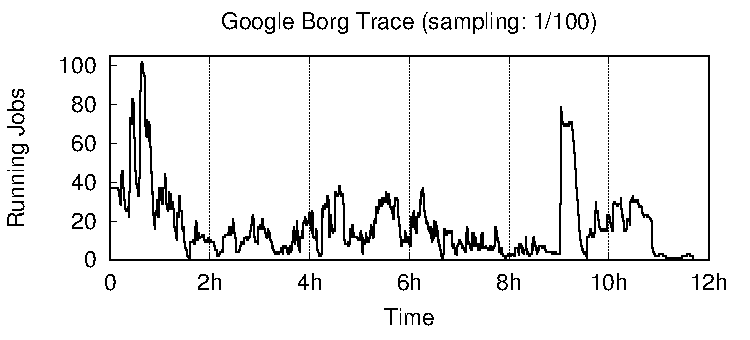
\includegraphics[]{figures/plots/borg/trace_dynamic}
  \caption{Initial 12 hours of the Google Borg Trace.}
  \label{fig:borg:dynamic}
\end{figure}

Figure~\ref{fig:borg:dynamic} shows the dynamics of the sampled workload in terms of concurrently executing jobs.
The sampled trace consists of $49,202$ jobs, with a peak of $102$ concurrent jobs, and an average job submission rate of $68.3$ jobs per minute.

For practical reasons, our experiments only consider the first $12$ hours of the trace, instead of the whole available period of 29 days.
Jobs that cross the 12-hour mark are killed abruptly.
We filter out jobs longer than $50$ minutes, as they represent less than $20\%$ of the jobs in the original trace and are not very meaningful given the 12-hour period consider.
Furthermore, in our sampling we only take into account the jobs that complete successfully.

\begin{figure}[t!]
  \centering
  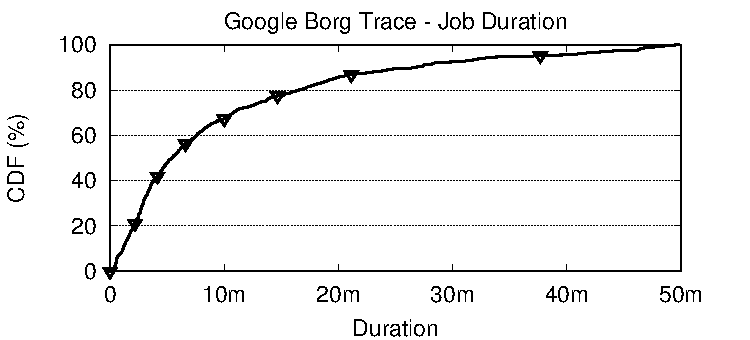
\includegraphics[]{figures/plots/borg/jobs_duration}
  \caption{Google Borg Trace: CDF of job durations.}
  \label{fig:borg:duration}
\end{figure}

Figure~\ref{fig:borg:duration} presents the duration of the jobs from the sampled trace as a \emph{cumulative distribution function} (CDF).
The considered jobs have a lifespan between $39\,s$ (the 5\emph{th} percentile) and $50\,m$ (the 100\emph{th} percentile).
Figure~\ref{fig:borg:resources} depicts the memory and CPU workload injected by the trace on our cluster.
We observe peak allocations of $42$ cores and $40\,GB$ of total memory required at any given time.

\begin{figure}[t!]
  \centering
  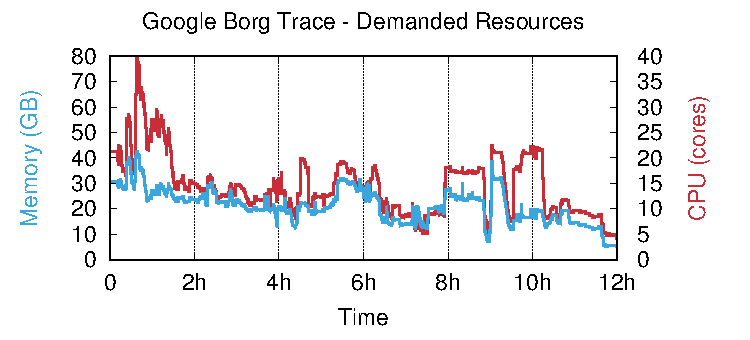
\includegraphics[]{figures/plots/borg/trace_resources}
  \caption{Google Borg Trace: demanded resources.}
  \label{fig:borg:resources}
\end{figure}

\subsection{Inside the \GP generations}
\label{subsec:eval:inside}

The \GP strategy involves the dispatch of containers and their following migration into the \emph{young} and the \emph{old} generations, according to the informations gathered during the automatic profiling phase.
Figure~\ref{fig:inside} shows the migrations occurring, during the first 2 hours, from/to the generations when \textsc{Docker Swarm} uses the \GP strategy.
We complement these results by looking at the total number of active hosts for each generation, as shown in Figure~\ref{fig:inside:generation}.
The sampled Borg trace triggers $131$ migrations from the nursery to the young and $50$ from the young to the old generation.
These results partially derive from the chosen configuration of monitoring periods.
We postpone to future work a full sensibility analysis of these parameters with respect to the Borg trace.

\begin{figure}[t!]
  \centering
  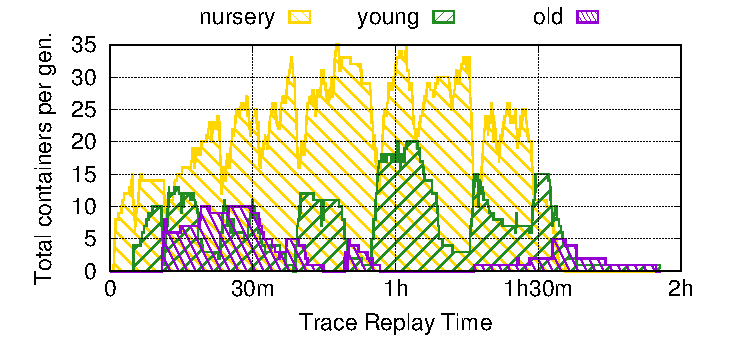
\includegraphics[]{figures/plots/containers/containers}
  \caption{Migration of containers between generations.}
  \label{fig:inside}
\end{figure}

\begin{figure}[t!]
  \centering
  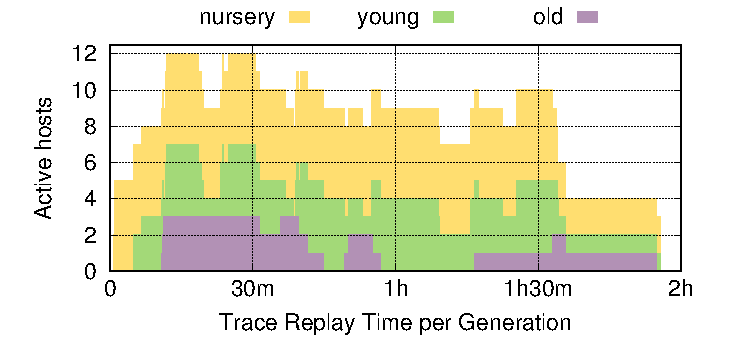
\includegraphics[]{figures/plots/containers/generation_hosts}
  \caption{Active hosts per generations.}
  \label{fig:inside:generation}
\end{figure}

While performing these experiments, we observe different replay timings---\emph{i.e.}, the time required to completely inject the Borg trace in our cluster---between the scheduling strategies under test.
Given the ideal duration of $1$ hour\vs{fix if get the results for 3 hours/12 hours/more}, the \emph{random} strategy completes in 1h19m54s, \emph{spread} in 1h02m42s, \emph{binpack} in 2h22m5s and finally the \GP strategy in 2h37m42s.
These differences can be explained by the different load on the \textsc{Docker} daemon running on the host VMs and in general the ability to load balance the containers across the hosts and VMs.
It is important to stress that these results correspond to the costs of injecting the Borg trace with our prototype, but do not directly reflect the system costs of scheduling in real conditions.
In particular, as we show in the following Section~\ref{subsec:eval:compl}, the four strategies are equivalent with respect to job completion times.


\subsection{Job completion time}
\label{subsec:eval:compl}

\begin{figure}[t!]
  \centering
  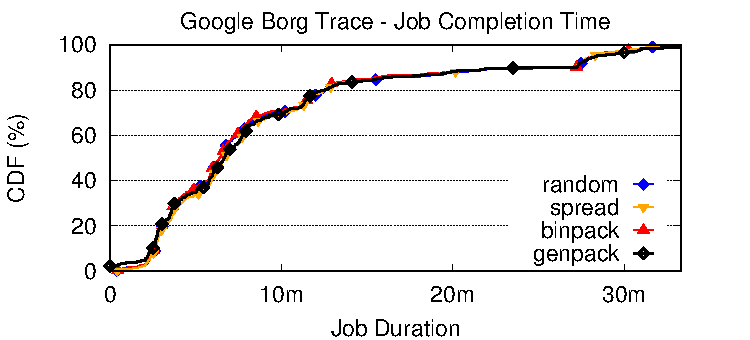
\includegraphics[]{figures/plots/completion/completion}
  \caption{Distribution (CDF) of job completion times.}
  \label{fig:completion}
\end{figure}

We compare the observed job completion time when using the default \textsc{Swarm} strategies against the \GP strategy.
Figure~\ref{fig:completion} shows that our approach does not impact negatively the executing time of the jobs.
The tested strategies result in the same long tail of few longer jobs as well as the same inflection point for the 90$^{th}$ percentile.
Instead, the $4$ strategies produce the same job completion distribution, and thus offer the same experience to the end-users of a \GP cluster.
Given the reported job completion times, we can conclude that \GP does not over-commit the cluster resources and rather offers a resource-efficient scheduling approach.

\subsection{Energy impact}
\label{subsec:eval:energy}

We demonstrate the interest of adopting the \GP strategy for a cloud data center by comparing its energy impact to the default \textsc{Swarm} strategies.
We rely on \textsc{BitWatts} probes to continuously report on the container's and node's power consumption.
Figure~\ref{fig:energy:joules} shows our results.
We present the normalized results against the \texttt{spread} baseline.
While the \texttt{binpack} strategy saves up $9\%$ of energy compared to \texttt{spread} default built-in strategy, \GP outperforms the existing strategies by saving $23\%$ of the cluster consumption.
These impressive results are due to the capability of \GP of \emph{i)} packing efficiently system containers onto a reduced number of nodes per generation and \emph{ii)} turning off unused nodes in each of the generations.
This result suggests that the \GP approach can lead to sensible savings for cloud data centers.
In particular, our evaluation based on real-world traces considers a large diversity of jobs' durations and profiles as well as incoming workloads, even though we could not inject the full Google Borg Trace.

We can also observe that the deployment of additional containers for monitoring the resource consumptions and computing the container envelopes does not penalize the power usage efficiency of \GP.
We can therefore conclude that \GP{} can achieve the same performances as existing scheduling strategies of \textsc{Docker Swarm}, but at a drastically reduced cost.

\begin{figure}[t!]
  \centering
  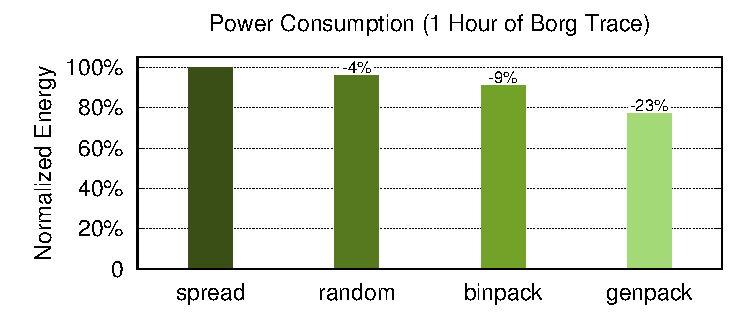
\includegraphics[]{figures/plots/energy/energy_joule}
  \caption{Normalized energy consumption.}
  \label{fig:energy:joules}
\end{figure}


% -*- root: Document.tex -*-

\chapter{Summary}
\label{chap:summ}

In this deliverable, we have presented the initial version of the specification, design and implementation of the \GP{} scheduler.
This scheduler is seamlessly working on top of \textsc{Docker Swarm}, and is so far fully compliant with it.

Efficient VM or container scheduling is particularly critical in cloud data centers to not only provide good performance, but also minimize the hardware resource required for running concurrent applications.
This can, in turn, reduce the costs of operating a cloud infrastructure and, importantly, reduce the associated energy footprint.
In particular, when efficiently packing containers on physical hosts, one can save significant amounts of energy by turning off unused servers.

\GP{} is a new scheduler for containers that borrows ideas from generational garbage collectors.
An original feature of \GP is that it does \emph{not} assume the properties of the containers and workloads to be known in advance.
It relies instead on runtime monitoring to observe the resource usage of containers while in the ``nursery''.
Containers are then run in a young generation of servers, which hold short-running jobs and experience relatively high turnaround.
This collection of servers can also be elastically expanded or shrunk to quickly adapt to the demand.
Long-running jobs are migrated to the old generation, which is composed of more stable and energy-efficient servers.
The containers in the old generation run for a long time and typically experience relatively even load, hence they can be packed in a very efficient way on the servers without need for frequent migrations.

We have implemented \GP in the context of \textsc{Docker Swarm} and evaluated it using a real-world trace.
Our comparison against \textsc{Swarm}'s built-in schedulers shows that \GP does not add noticeable overheads while providing more efficient container packing, which can result in important energy savings.

Our perspectives for \GP includes a careful sensitivity analysis of key parameters like the $k$-means value or the scheduling period.
We also plan to evaluate the performances of \GP in a long-running deployment evolving not only CPU- and memory- intensive containers, but also network- and disk-intensive ones.

% -*- root: Document.tex -*-

\chapter{User Manual}
\label{chap:usermanual}

\GP{} aims to work seamlessly on top of \textsc{Docker} through a manager of a legacy standalone \textsc{Docker Swarm} cluster.
That means that you can refer to the documentation of \textsc{Docker}\footnote{\textsc{Docker} CLI user guide: \url{https://docs.docker.com/engine/reference/commandline/cli/}.} and \textsc{Docker Swarm}\footnote{Legacy standalone \textsc{Docker Swarm} documentation: \url{https://docs.docker.com/swarm/overview/}.} for any details to use the \textsc{Docker} CLI for deploying containers on a cluster.

First of all, a \textsc{Docker Swarm} cluster have to be deployed (cf. Section~\ref{sec:clustersetup}), and \GP{} have to be run (cf. Section~\ref{sec:genpacksetup}).

The only requirement to use \GP{} when you are deploying some containers is to deploy them first on the generation \texttt{nursery}.
For that, a constraint filter\footnote{\textsc{Docker Swarm} constraint filters documentation: \url{https://docs.docker.com/swarm/scheduler/filter/\#use-a-constraint-filter}.}, for targeting the wanted generation, has to be given in the command of container creation, \textit{e.g.} (assuming that the \textsc{Docker Swarm} manager can be reached on the address \texttt{tcp://0.0.0.0:2380}):

\begin{lstlisting}[language=bash, basicstyle=\small]
$ docker -H :2380 run --name nginx -e constraint:generation==nursery -d nginx
\end{lstlisting}

Then the container \texttt{nginx} is deployed on a node of the generation \texttt{nursery}.
It will be migrated accross the different generations by \GP{}'s generation cycles.


% -*- root: Document.tex -*-

\section{Infrastructure}
\label{sec:infrastructure}

\GP{} is running on top of a \textsc{Docker Swarm} cluster.
To build this one, you need a set of hosts reachable by SSH.
Each host has to have a \textsc{Docker} daemon running and binded on the address \texttt{tcp://0.0.0.0:2375}.


\newpage

% -*- root: Document.tex -*-

\section{Cluster Setup}
\label{sec:clustersetup}

A tiny CLI tool has been implemented to setup easily a \textsc{Docker Swarm} cluster.
This one can be downloaded at \remoteswarmmanagerrepo{}.
Once the configuration for the different hosts used to build the cluster is given (cf. Subsection~\ref{subsec:clustersetup:config}), the CLI can be used to build a \textsc{Docker Swarm} cluster (cf. Subsection~\ref{subsec:clustersetup:manage}).
Note that the example of configuration given here is present in the file \texttt{config.yml.example}: you can copy this file to \texttt{config.yml} and modify it with your own configuration.

When the CLI is called without any command, it returns the list of the available ones:

\begin{lstlisting}[basicstyle=\small]
$ ./remote_swarm_manager.rb
Welcome to the remote Swarm manager

Version: 0.1.0
Use one or several (you can chain them) of the following commands:

- help		Print this usage notice
- version	Print used version of Swarm
- login		Print command to login on each cluster node (manually)
- pull		Pull image given in arg, Swarm image by default
- create	Create a Swarm cluster
- create-nodes	Create Docker nodes
- remove	Remove the current cluster
- ps		Print containers on swarm docker manager
- info		Print infos about swarm docker manager
- monitor	Run cAdvisor on cluster nodes for monitoring
- rm-monitor	Remove cAdvisor and PowerAPI on cluster nodes
- hostnames	Set hostname for each node
- export-key	Export your public key on each VM: export-key [filepath]
- swarm-version	Print used version of Swarm
- ping		Check if connexions for each VM are well configured

For example:	 ./remote_swarm_manager.rb remove monitor create run
\end{lstlisting}

% -*- root: Document.tex -*-

\subsection{Requirements and dependencies}
\label{subsec:clustersetup:requirements}

The CLI requires \textsc{Ruby} v. \texttt{2.3.1}.
If you don't have this version of \textsc{Ruby} installed on your system, you can use \textsc{RVM}\footnote{Install \textsc{RVM}, Ruby Version Manager: \url{https://rvm.io/}.} to easily install it.

The CLI uses some dependencies defined in the file \texttt{Gemfile}. You need to use \textsc{Bundler}\footnote{\textsc{Bundler}, package manager for \textsc{Ruby}: \url{http://bundler.io/}.} to install them.
It can be installed with the command:

\begin{lstlisting}[language=bash, basicstyle=\small]
$ gem install bundler
\end{lstlisting}

Using \textsc{Bundler}, you can install all \textsc{Ruby} dependencies with the command:

\begin{lstlisting}[language=bash, basicstyle=\small]
$ bundle install
\end{lstlisting}

Some of the \textsc{Ruby} dependencies have to be built as native extensions.
For that, \textsc{Bundler} will use \textsc{Make} and \textsc{GCC}: be sure to have those installed on your systems before running the command above.


% -*- root: Document.tex -*-

\subsection{Configuration}
\label{subsec:clustersetup:config}

The configuration has to be given into the YAML file \texttt{config.yml} at the root of tool's code.
This file has to be build like in the example~\ref{remote-swarm-manager-config}.
All configurations options are detailed below.

\begin{minipage}{\linewidth} %avoid splitting
% \vspace{10pt}
\begin{lstlisting}[language=YAML,caption={Configuration file example for \textsc{RemoteSwarmManager} CLI.},label=remote-swarm-manager-config][t]
ssh:
  user: 'host_user'
  identity_file: 'path/to/ssh_keys/id_rsa'
  public_key_file: 'path/to/ssh_keys/id_rsa.pub'
  proxy:
    user: 'proxy_user'
    host: 'proxy_host'

cluster:
  manager: 172.16.0.30
  manager_docker_port: 2380
  node_docker_port: 2380
  nodes:
    -
      ip: 172.16.0.2
      cpu: 4
      name: 'nursery-node-1'
      group: 'nursery'
    -
      ip: 172.16.0.4
      cpu: 4
      name: 'young-node-1'
      group: 'young'
    -
      ip: 172.16.0.6
      cpu: 8
      name: 'tenured-node-1'
      group: 'tenured'

swarm:
  image: swarm:1.2.0
  strategy: spread
  host_image: docker:1.12.0-rc3-dind
\end{lstlisting}
\end{minipage}

\subsubsection{SSH options}

The CLI is using the protocol \textsc{SSH} to access to the different hosts of your cluster.

\begin{itemize}
  \item \texttt{user} (\emph{mandatory}): the user you want to use to connect to hosts;
  \item \texttt{identity\_file} (\emph{mandatory}): the path to the private key to use to connect to hosts;
  \item \texttt{public\_key\_file} (\emph{optional}): the path to the public key to use to connect to hosts - required only for using CLI's feature for exporting a public key on remote hosts;
  \item \texttt{proxy} (\emph{optional}): the proxy to use to reach the different hosts - required only to use a proxy, it will use the same key than the one for hosts.
\end{itemize}

\subsubsection{Cluster options}

Here are defined all the parameters related to the infrastructure of the cluster:

\begin{itemize}
  \item \texttt{manager} (\emph{mandatory}): IP address of host where the \textsc{Docker Swarm} manager will be deployed;
  \item \texttt{manager\_docker\_port} (\emph{mandatory}): port where the \textsc{Docker Swarm} manager will listen;
  \item \texttt{node\_docker\_port} (\emph{mandatory}): port where the \textsc{Docker Swarm} nodes will listen;
  \item \texttt{nodes} (\emph{mandatory}): the list of the \textsc{Docker Swarm} nodes to set in the cluster, with for each:
  \begin{itemize}
    \item \texttt{ip} (\emph{mandatory}): IP address of the host;
    \item \texttt{cpu} (\emph{mandatory}): number of CPUs of the host;
    \item \texttt{name} (\emph{mandatory}): name to give to the host;
    \item \texttt{group} (\emph{mandatory}): generation which the node is belonging to, either \texttt{nursery}, \texttt{young} or \texttt{tenured}.
  \end{itemize}
\end{itemize}

\subsubsection{Swarm options}

Finally, few parameters about \textsc{Docker Swarm} have to be set:

\begin{itemize}
  \item \texttt{image} (\emph{mandatory}): the image of \texttt{Docker Swarm} to use;
  \item \texttt{strategy} (\emph{mandatory}): the strategy of scheduling to give to \texttt{Docker Swarm} - it will be used only to schedule nodes on the nursery;
  \item \texttt{host\_image} (\emph{mandatory}): the image of \texttt{Docker} to use on the nodes.
\end{itemize}


% -*- root: Document.tex -*-

\subsection{Manage a cluster}
\label{subsec:clustersetup:manage}

We are assuming that your hosts are all reachable by SSH from the CLI.
You can ensure that by running:

\begin{lstlisting}[language=bash, basicstyle=\small]
$ ./remote_swarm_manager.rb ping
\end{lstlisting}

Once the configuration of the hosts to use for creating the cluster has been given, here are the few steps needed to create a cluster:

\begin{itemize}
  \item \emph{Create nodes}: this command will be create the nodes to use in the \textsc{Docker Swarm} cluster, by deploying an image of \textsc{Docker} on the \textsc{Docker} daemon of each host:
    \begin{lstlisting}[language=bash, basicstyle=\small]
  $ ./remote_swarm_manager.rb create-nodes
    \end{lstlisting}
  \item \emph{Create the cluster}: this command will deploy the \textsc{Docker Swarm} cluster:
    \begin{lstlisting}[language=bash, basicstyle=\small]
  $ ./remote_swarm_manager.rb create
    \end{lstlisting}
  \item \emph{Monitor the cluster}: this command will deploy the services responsible of monitoring resources:
    \begin{lstlisting}[language=bash, basicstyle=\small]
  $ ./remote_swarm_manager.rb monitor
    \end{lstlisting}
\end{itemize}

All these commands can be run at once:

\begin{lstlisting}[language=bash, basicstyle=\small]
    $ ./remote_swarm_manager.rb create-nodes create monitor
\end{lstlisting}

If you want to recreate a cluster, use the command \texttt{remove} before, \textit{e.g.}:

\begin{lstlisting}[language=bash, basicstyle=\small]
    $ ./remote_swarm_manager.rb remove create-nodes create monitor
\end{lstlisting}



\newpage

% -*- root: Document.tex -*-

\section{Genpack Setup}
\label{sec:genpacksetup}

\GP{} can be downloaded at \genpackschedulerrepo{}.

\GP{} is requiring a well configured \textsc{Docker Swarm} cluster and the monitoring system deployed on the cluster (cf. Subsection~\ref{subsec:clustersetup:manage}).



% -*- root: Document.tex -*-

\subsection{Requirements and dependencies}
\label{subsec:genpacksetup:requirements}

Requirements and the installation of dependencies for \textsc{Genpack} are exactly like those described in Subsection~\ref{subsec:clustersetup:requirements}.


% -*- root: Document.tex -*-

\subsection{Configuration}
\label{subsec:genpacksetup:config}

\subsubsection{Global Configuration}

The global configuration has to be given into the YAML file \texttt{config.yml} at the root of \GP{}'s code.
This file has to be build like in the example~\ref{genpack-scheduler-config}.
All configurations options are detailed below.

\begin{minipage}{\linewidth} %avoid splitting
% \vspace{10pt}
\begin{lstlisting}[language=YAML,caption={Configuration file example for \GP{} scheduler.},label=genpack-scheduler-config][t]
genpack:
  docker_url: "tcp://localhost:2375"
  swarm_url: "tcp://localhost:2380"
  redis_host: 'localhost'
  redis_port: 6379
  redis_docker_image: 'redis:3.2.1-alpine'
  generations:
    - nursery
    - young
    - tenured
\end{lstlisting}
\end{minipage}

\begin{itemize}
  \item \texttt{docker\_url} (\emph{optional}): the url to reach the \textsc{Docker} daemon on manger host;
  \item \texttt{swarm\_url} (\emph{optional}): the url to reach the \textsc{Docker Swarm} manager;
  \item \texttt{redis\_host} (\emph{optional}): the address of the \textsc{Redis} server;
  \item \texttt{redis\_docker\_image} (\emph{optional}): the image to use for deploying the \textsc{Redis} server;
  \item \texttt{swarm\_url} (\emph{optional}): the url to reach the \textsc{Docker Swarm} manager;
  \item \texttt{generations} (\emph{mandatory}): the list of the different generations - its order is important because it will define the order between generations.
\end{itemize}

All mandatory values above are set by default to the ones given in the example~\ref{genpack-scheduler-config}.

\subsubsection{Generation Cycles Configuration}

The cycles of migration between the generations are executed like some tasks.
These tasks are some jobs performed by \textsc{Resque}\footnote{\textsc{Resque} is a \textsc{Redis}-backed \textsc{Ruby} library for creating background jobs, placing them on multiple queues, and processing them later: \url{https://github.com/resque/resque}.} workers and launched by a task scheduler, \textsc{Resque Scheduler}\footnote{\textsc{Resque Scheduler}, light-weight job scheduling system built on top of \textsc{Resque}: \url{https://github.com/resque/resque-scheduler}.}.
The frequency of generation cycles is configured in the file \texttt{config/resque\_schedule.yml} (cf. Listing~\ref{resque-scheduler-config}), using the \textsc{Crontab} syntax\footnote{\textsc{Crontab} Quick Reference: \url{http://www.adminschoice.com/crontab-quick-reference}.}.
In the example given here, each \emph{GenerationCycle} from \texttt{nursery} to \texttt{young} generations is executed every 5 minutes, each one from \texttt{young} to \texttt{tenured} generations each 10 minutes.

\begin{minipage}{\linewidth} %avoid splitting
% \vspace{10pt}
\begin{lstlisting}[language=YAML,caption={Configuration file for \textsc{Resque Scheduler}.},label=resque-scheduler-config][t]
  generation_nursery_cycle:
    cron: "*/5 * * * *"
    class: GenerationCycle
    description: "Run a cycle on generation nursery"
    args: nursery

  generation_young_cycle:
    cron: "*/10 * * * *"
    class: GenerationCycle
    description: "Run a cycle on generation young"
    args: young
\end{lstlisting}
\end{minipage}


% -*- root: Document.tex -*-

\subsection{Run \GP{}}
\label{subsec:genpacksetup:run}

We are assuming that your \textsc{Docker Swarm} manager, the \textsc{Docker} daemon from your manager host, the servers \textsc{Redis} and \textsc{InfluxDB} are all reachable from where you are launching \GP{}.
Typically, \GP{} is launched on the \textsc{Docker Swarm} manager host, but you can also launch it remotely if each service is reachable from thre (you can eventually open some SSH tunnels for that).

Once all the requirements described above are checked, run \GP{} from the root of its code directory with the command:

\begin{lstlisting}[basicstyle=\small]
$ bundle exec rake genpack:init
\end{lstlisting}

Then you can follow \GP{}'s logs from the file \texttt{log/genpack.log}.

You can now run some containers when it is explained at the beginning of this chapter~\ref{chap:usermanual}.




\begin{raggedright}

\bibliographystyle{IEEEtran}
\bibliography{Document.bib}

\end{raggedright}

\end{document}
